\documentclass[a4paper,12pt]{article}

\usepackage[utf8]{inputenc}      % Кодировка
\usepackage[T2A]{fontenc}        % Кодировка
\usepackage[russian]{babel}      % Поддержка русского языка
\usepackage{amsmath,amssymb}     % Математические символы и окружения
\usepackage{geometry}            % Пакет для задания полей страницы
\usepackage{graphicx}            % Для вставки рисунков (графиков)
\usepackage{wrapfig}             % Обтекание рисунков/таблиц текстом
\usepackage{float}               % Улучшенное размещение плавающих объектов (рисунков/таблиц)
\geometry{left=2cm,right=2cm,top=2cm,bottom=2cm}

\begin{document}
\begin{titlepage}
    \centering
    {\large Федеральное государственное автономное образовательное учреждение\par}
    {\large высшего образования\par}
    {\bfseries САНКТ-ПЕТЕРБУРГСКИЙ НАЦИОНАЛЬНЫЙ ИССЛЕДОВАТЕЛЬСКИЙ УНИВЕРСИТЕТ ИТМО\par}
    {\bfseries Факультет систем управления и робототехники\par}
    \vfill
    {\Large \bfseries Отчёт по лабораторной работе №1\par}
    {\Large \bfseries по дисциплине <<Математическая статистика>>\par}
    {\Large Вариант 3\par}
    \vfill
    
    \begin{flushright}
        Студент: Сайфуллин Д.Р. \\
        Поток: Мат Стат 22 \\
        Преподаватель: Шкваренко А.А.
    \end{flushright}
    \vfill
    Санкт-Петербург \\
    2025 г.
\end{titlepage}

\section*{Задание 1}
Для выполнения данного задания необходимо выбрать непрерывное распределение, у которого существуют первые четыре момента. Далее требуется экспериментально убедиться в асимптотической нормальности выборочного среднего, выборочной дисперсии и выборочной медианы (квантиль порядка $0.5$). Также нужно проверить выполнение:
\[
    n\,F\bigl(X_{(2)}\bigr)
    \ \xrightarrow{} U_1 \sim \Gamma(2,1),
    \quad
    n\Bigl(1 - F\bigl(X_{(n)}\bigr)\Bigr)
    \ \xrightarrow{} U_2 \sim \Gamma(1, 1) = \mathrm{Exp}(1).
\]
где $X_{(2)}$ --- вторая порядковая статистика, $X_{(n)}$ --- максимальная порядковая статистика, а $F$ --- функция распределения выбранного закона.

В данной работе возьмем распределение $\Gamma(\alpha=3,\theta=2)$. Далее $M = 1000$ раз сгенерируем выборки объемом $n = 1000$.
Для каждой выборки рассчитаем выборочное среднее, выборочную дисперсию, медиану, найдем второй элемент в выборке, а также максимальное значение. Построим гистограммы и сравним их с теоретическими значениями распределения.
\begin{figure}[H]
    \centering
    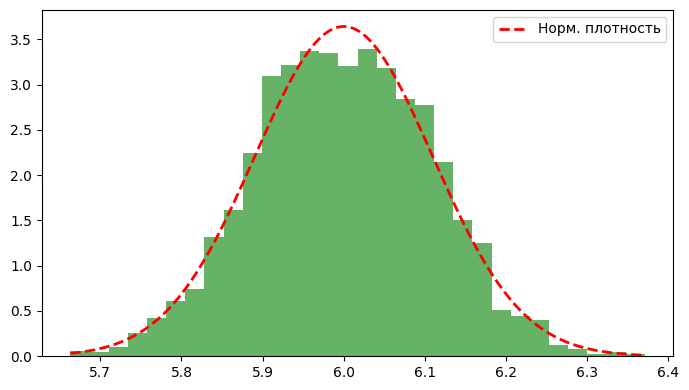
\includegraphics[width=0.7\textwidth]{images/hist_mean.png}
    \caption{Гистограмма выборочного среднего.}
    \label{fig:hist_mean}
\end{figure}
Как видно на рис.~\ref{fig:hist_mean}, гистограмма имеет выраженную колоколообразную форму и хорошо согласуется с наложенной нормальной кривой. Пик распределения расположен близко к теоретическому среднему, а «хвосты» симметричны относительно этого пика. 
\begin{figure}[H]
    \centering
    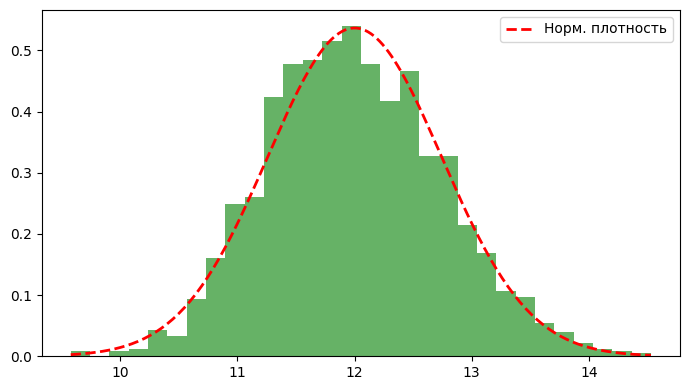
\includegraphics[width=0.7\textwidth]{images/hist_var.png}
    \caption{Гистограмма выборочной дисперсии.}
    \label{fig:hist_var}
\end{figure}
Распределение выборочной дисперсии тоже выглядит близким к нормальному, хотя иногда оно бывает чуть более «асимметричным», чем выборочное среднее. Максимум гистограммы находится около теоретической дисперсии, и «хвосты» распределения сравнительно симметричны.
\begin{figure}[H]
    \centering
    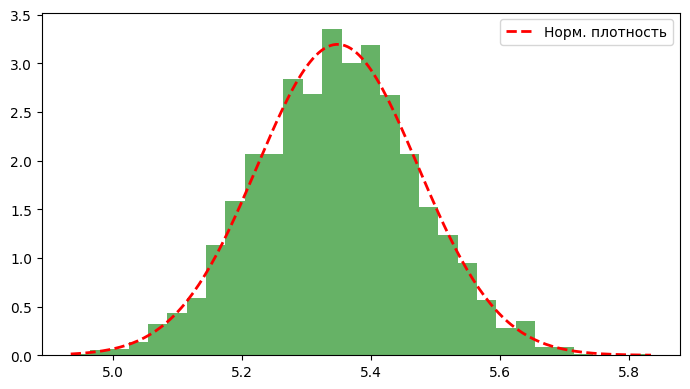
\includegraphics[width=0.7\textwidth]{images/hist_med.png}
    \caption{Гистограмма выборочной квантили порядка 0,5.}
    \label{fig:hist_med}
\end{figure}
Гистограмма медианы показывает, что центр графика находится рядом с истинной медианой, что означает, что при большом объёме выборки медиана почти всегда получается около этого значения.

Вычислим теоретические значения мат. ожидания, дисперсии и медианы для гамма-распределения \(\Gamma(3,2)\) с параметрами 
\(\alpha = 3\) и \(\theta = 2\). Тогда:
\[
\mathbb{E}[X] \;=\; \alpha\,\theta \;=\; 3 \times 2 \;=\; 6,
\]
\[
\mathrm{D}[X] \;=\; \alpha\,\theta^2 \;=\; 3 \times (2)^2 \;=\; 12.
\]
Точная формула для медианы гамма-распределения в элементарных функциях не выражается, поэтому её находят через обратную функцию распределения (квантильную функцию) при уровне $0.5$:
\[
\mathrm{median}[X] \;=\; F^{-1}(0.5).
\]
С использованием пакета \texttt{scipy.stats} в Python вычисляем приближенное значение:
\[
\mathrm{median}[X] \;\approx\; 5.348.
\]
Выведем численные результаты мат. ожидания, дисперсии и медианы для анализа:
\begin{table}[H]
    \centering
    \begin{tabular}{|l|ccc|}
        \hline
        & $\overline{X}$ & $S^2$ & median \\ 
        \hline
        Среднее по $M$  & 5.999 & 11.991 & 5.348 \\
        Дисперсия по $M$ & 0.012 & 0.573 & 0.016 \\
        Медиана по $M$   & 5.999 & 11.957 & 5.348 \\
        \hline
        Теор. значение & 6 & 12 & 5.348 \\
        \hline
    \end{tabular}
    \caption{Числовые результаты по распределениям оценок}
\end{table}
Все три гистограммы (для выборочного среднего, выборочной дисперсии и медианы) демонстрируют «колоколообразную» форму, хорошо согласующуюся с наложенной нормальной плотностью. Это свидетельствует об асимптотической нормальности рассмотренных оценок. Дополнительно, таблица с численными результатами показывает, что средние значения этих оценок (по всем сгенерированным выборкам) близки к теоретическим (мат. ожидание около 6, дисперсия около 12, медиана около 5.35). При этом «дисперсия по М» для выборочной дисперсии (около 0.57) отражает разброс самой оценки \(S^2\) между повторными экспериментами, а не расхождение с теоретическим \( \mathrm{D}[X]=12 \). Таким образом, и визуальный, и численный анализ подтверждают корректность генерации выборок, согласие с теорией и асимптотическую нормальность статистик.

Теперь необходимо экспериментально убедиться в сходимости следующих величин к гамма-распределениям:
\[
U_1 \;=\; n\,F\bigl(X_{(2)}\bigr) \;\;\xrightarrow{}\;\; \Gamma(2,1),
\]
\[
U_2 \;=\; n\,\bigl(1 - F\bigl(X_{(n)}\bigr)\bigr) \;\;\xrightarrow{}\;\; \Gamma(1,1),
\]
где $X_{(2)}$ --- вторая порядковая статистика (второе по величине значение в выборке), $X_{(n)}$ --- максимум (наибольшее значение выборки), а $F(x)$ --- функция гамма-распределения.
Для каждой выборки найдем $X_{(2)}$ и $X_{(n)}$, то есть отсортируем выборку и возьмем второй и максимальный элементы. Подставим их в формулы и построим гистограммы для массивов $\{U_1^{(i)}\}$ и $\{U_2^{(i)}\}$. Для визуального сравнения наложим теоретические плотности $\Gamma(2,1)$ и $\Gamma(1,1)$ соответственно.
\begin{figure}[H]
    \centering
    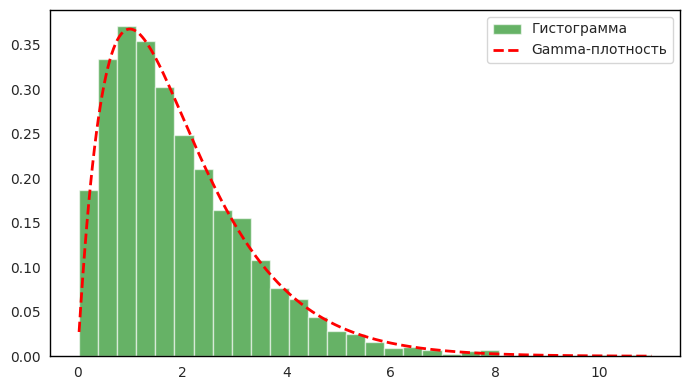
\includegraphics[width=0.48\textwidth]{images/U1.png}
    \quad
    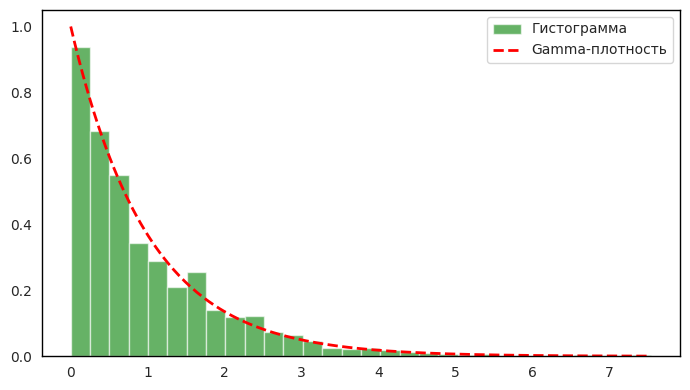
\includegraphics[width=0.48\textwidth]{images/U2.png}
    \caption{Гистограммы $U_1 = n\,F(X_{(2)})$ (слева) и $U_2 = n\,(1-F(X_{(n)}))$ (справа) 
             с наложенными плотностями $\Gamma(2,1)$ и $\Gamma(1,1)$ соответственно.}
    \label{fig:U1_U2_gamma}
\end{figure}
Как видно из рисунка, в обоих случаях распределения гистограмм близки к теоретическим кривым гамма-распределения. При достаточно большом объёме выборки $n$ и количестве повторений $M$ наблюдается хорошее совпадение с соответствующими плотностями.

\section*{Задание 2}
В файле \texttt{cars93.csv} содержатся данные о ~93 моделях автомобилей: их мощность (\texttt{Horsepower}), тип (\texttt{Type}), производитель (\texttt{Manufacturer}) и другие характеристики. Для выполнения задания необходимо загрузить датасет и ответить на следующие вопросы:
\begin{enumerate}
    \item Определим, какие типы автомобилей (\texttt{Type}) представлены в датасете, а также найдем наиболее и наименее распространённый тип.
    \item Для мощности (\texttt{Horsepower}) вычислить (для всех автомобилей и для каждого типа отдельно): 
          \begin{itemize}
              \item выборочное среднее, 
              \item выборочную дисперсию, 
              \item выборочную медиану, 
              \item межквартильный размах.
          \end{itemize}
    \item Построить (для всех автомобилей и для каждого типа отдельно):
          \begin{itemize}
              \item график эмпирической функции распределения,
              \item гистограмму,
              \item box-plot.
          \end{itemize}
\end{enumerate}

С помощью библиотеки \texttt{pandas} загрузим датасет и выведем какие типы автомобилей представлены и их количество. Далее найдем наиболее и наименее распространенный тип автомобилей:
\begin{table}[H]
    \centering
    \begin{tabular}{|l|c|}
        \hline
        \textbf{Тип} & \textbf{Количество} \\
        \hline
        \texttt{Midsize} & 22 \\
        \texttt{Small}   & 21 \\
        \texttt{Compact} & 16 \\ 
        \texttt{Sporty}  & 14 \\
        \texttt{Large}   & 11 \\
        \texttt{Van}     & 9  \\
        \hline
    \end{tabular}
    \caption{Результаты программы}
\end{table}
Как видно по таблице наиболее распространённым типом является Midsize, а наименее распространённый --- Van.

Теперь вычислим для мощности (\texttt{Horsepower}) выборочное среднее, выборочную дисперсию, выборочную медиану и межквартильный размах для всех автомобилей: 
\begin{table}[H]
    \centering
    \begin{tabular}{|l|c|}
        \hline
        \textbf{Статистика} & \textbf{Значение}  \\ 
        \hline
        $\overline{X}$  & 143.83 \\
        $S^2$ & 2743.08 \\
        $Median$ & 140.00 \\
        $IQR$ & 67.00 \\
        \hline
    \end{tabular} 
    \caption{Статистики для всей совокупности}
\end{table}
И для каждого типа отдельно:
\begin{table}[H]
    \centering
        \begin{tabular}{|l|c|c|c|c|c|c|}
        \hline
            & \texttt{Compact} & \texttt{Large} & \texttt{Midsize} & \texttt{Small} & \texttt{Sporty} & \texttt{Van} \\
        \hline
        $\overline{X}$ & 131.00 & 179.45 & 173.09 & 91.00 & 160.14 & 149.44 \\
        $S^2$          & 518.53 & 477.07 & 2756.09 & 447.60 & 5536.29 & 370.28 \\
        $Median$       & 132.00 & 170.00 & 169.00  & 90.00  & 147.50  & 151.00 \\
        $IQR$          & 33.25  & 25.00  & 69.00   & 21.00  & 72.25   & 23.00  \\
        \hline
        \end{tabular}
    \caption{Статистики для каждого типа отдельно}
\end{table}

\begin{figure}[H]
    \begin{minipage}{0.49\textwidth}
        \centering
        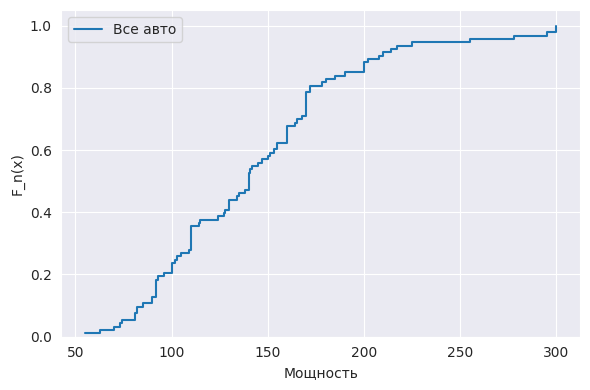
\includegraphics[width=\textwidth]{images/ecdf_all.png}
    \end{minipage}
    \begin{minipage}{0.49\textwidth}
        \centering
        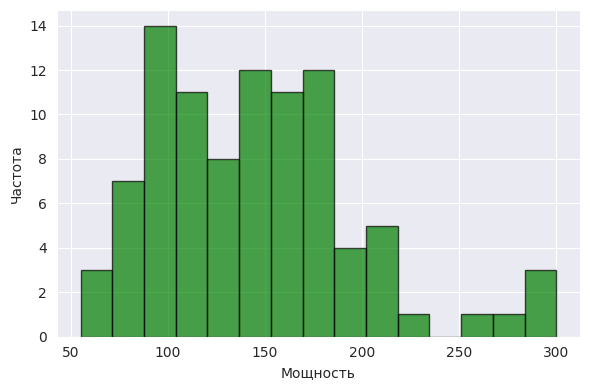
\includegraphics[width=\textwidth]{images/hist_all.png}
    \end{minipage}
    \begin{minipage}{\textwidth}
        \centering
        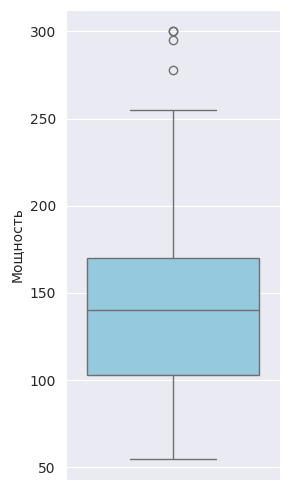
\includegraphics[width=0.3\textwidth]{images/boxplot_all.png}
    \end{minipage}
    \centering          
    \caption{Графики мощности (\texttt{Horsepower}) для всех автомобилей: эмпирическая функция распределения, гистограмма, box-plot.}
    \label{fig:allcars}
\end{figure}
Построенные графики показывают одну информацию, но в разных визуальных формах. Разберем каждый из них:
\begin{itemize}
    \item \textbf{Эмпирическая функция распределения.} Ступенчатая кривая показывает, как распределены автомобили по мощности. Например, по оси $x$ можно примерно оценить, что около 50\,\% автомобилей (то есть медиана) имеют мощность порядка 130--140. Видно, что кривая накапливается постепенно до значений около 200~л.\,с., затем есть относительно небольшой «скачок» к 250--300~л.\,с., где находятся немногие машины.
    \item \textbf{Гистограмма.} Наиболее массовый диапазон мощностей --- примерно 90--170~л.\,с. Есть «пик» в районе 100--110~л.\,с. и 140--150~л.\,с., а также заметный разрыв в интервале 210--240~л.\,с. Небольшое количество автомобилей имеет мощность выше 250~л.\,с.
    \item \textbf{Box-plot.} Отчётливо видно, что медиана находится примерно в диапазоне 130--140~л.\,с. Верхняя и нижняя границы «ящика» соответствуют первому и третьему квартилю. В данной выборке есть несколько выбросов (точки сверху), то есть модели с существенно большей мощностью (более 250~л.\,с.).
\end{itemize}
Теперь построим графики распределения мощности по типам автомобилей
\begin{figure}[H]
    \centering
    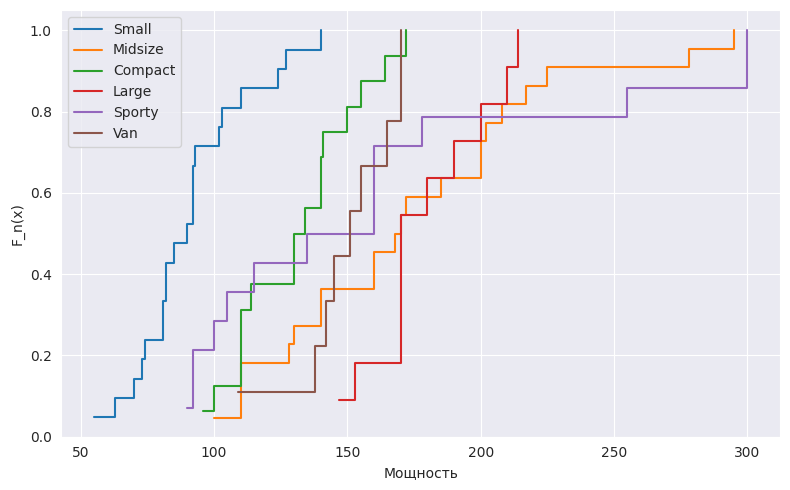
\includegraphics[width=0.75\textwidth]{images/ecdf_types.png}
    \caption{Эмпирические функции распределения мощности по каждому типу авто.}
    \label{fig:ecdf_types}
\end{figure}

\noindent
На рис.~\ref{fig:ecdf_types} представлены эмпирические функции распределения         для каждого типа:
\begin{itemize}
    \item Кривая для \texttt{Small} смещена влево (большая часть значений ниже 120~л.\,с.).
    \item \texttt{Midsize} и \texttt{Sporty} имеют более «длинный хвост» вправо: некоторые модели достигают 250--300~л.\,с.
    \item \texttt{Compact} и \texttt{Van} занимают промежуточное положение между \texttt{Small} и \texttt{Large}.
\end{itemize}

Ниже приведены гистограммы для каждого типа автомобиля по отдельности, позволяющие более детально увидеть характер распределения внутри группы.

\begin{figure}[H]
    \centering
    \begin{minipage}{0.45\textwidth}
        \centering
        \includegraphics[width=\textwidth]{images/hist_small.png}
        \caption{\texttt{Small}}
    \end{minipage}
    \quad
    \begin{minipage}{0.45\textwidth}
        \centering
        \includegraphics[width=\textwidth]{images/hist_midsize.png}
        \caption{\texttt{Midsize}}
    \end{minipage}
    
    \begin{minipage}{0.45\textwidth}
        \centering
        \includegraphics[width=\textwidth]{images/hist_compact.png}
        \caption{\texttt{Compact}}
    \end{minipage}
    \quad
    \begin{minipage}{0.45\textwidth}
        \centering
        \includegraphics[width=\textwidth]{images/hist_large.png}
        \caption{\texttt{Large}}
    \end{minipage}

    \begin{minipage}{0.45\textwidth}
        \centering
        \includegraphics[width=\textwidth]{images/hist_sporty.png}
        \caption{\texttt{Sporty}}
    \end{minipage}
    \quad
    \begin{minipage}{0.45\textwidth}
        \centering
        \includegraphics[width=\textwidth]{images/hist_van.png}
        \caption{\texttt{Van}}
    \end{minipage}
\end{figure}
Гистограммы показывают, что распределение мощности внутри каждого типа автомобиля имеет свои особенности:
\begin{itemize}
    \item Типы \texttt{Small} и \texttt{Compact} характеризуются сравнительно невысокой мощностью (часто менее 140--150~л.\,с.), причём у \texttt{Small} заметен минимум около 50~л.\,с.
    \item \texttt{Midsize}, \texttt{Large} и \texttt{Sporty} имеют более широкий разброс: есть модели как с мощностью около 100~л.\,с., так и с показателями свыше 200--250~л.\,с.
    \item У \texttt{Van} мощность в основном сосредоточена в интервале 130--170~л.\,с. и редко выходит за его пределы.
    \item В целом, если сравнить медианы (см. box-plot), наиболее «слабомощными» оказываются автомобили \texttt{Small}, а наиболее «сильными» --- отдельные модели из \texttt{Midsize} и \texttt{Sporty}.
\end{itemize}

\begin{figure}[H]
    \centering
    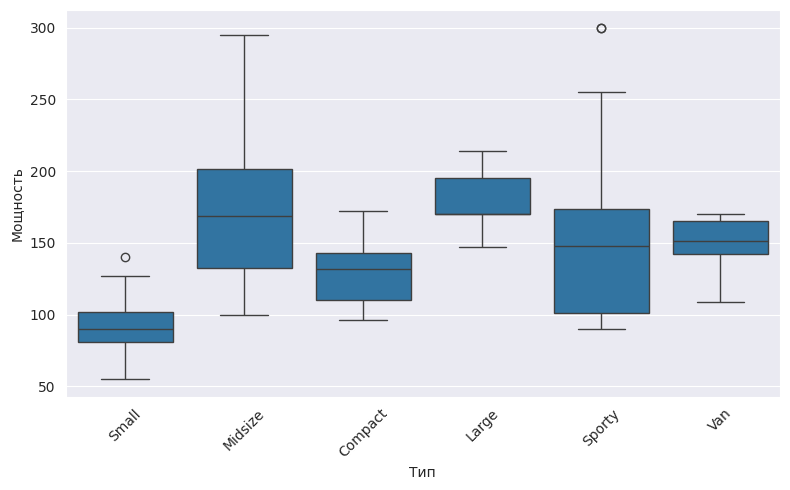
\includegraphics[width=0.75\textwidth]{images/boxplot_types.png}
    \caption{Box-plot распределения мощности по каждому типу автомобиля.}
    \label{fig:boxplot_types}
\end{figure}

\noindent
На рис.~\ref{fig:boxplot_types} видно, что распределение мощности существенно варьируется в зависимости от типа авто. Например:
\begin{itemize}
    \item \texttt{Small} --- имеют сравнительно невысокую мощность (медиана около 90--100~л.\,с.), при этом присутствует один автомобиль с ещё более низкой мощностью (выброс).
    \item \texttt{Midsize} --- разброс достаточно велик, верхняя «уса» достигает 300~л.\,с., а медиана лежит в районе 170~л.\,с.
    \item \texttt{Compact} --- в среднем чуть меньше 140~л.\,с., заметно более «скромный» разброс, чем у \texttt{Midsize} или \texttt{Sporty}.
    \item \texttt{Large} --- медиана около 170--180~л.\,с. и довольно короткие усы, т.\,е. большая часть значений сгруппирована ближе к центру.
    \item \texttt{Sporty} --- имеет значительную вариативность: нижняя граница может быть порядка 90--100~л.\,с., тогда как верхние значения превышают 250~л.\,с. (выброс).
    \item \texttt{Van} --- мощность в среднем около 150~л.\,с. с довольно узким разбросом.
\end{itemize}

\section*{Вывод}

По результатам выполнения двух заданий можно сделать следующие выводы:

\begin{enumerate}
    \item \textbf{Задание 1.}\\
    Было выбрано распределение (гамма-распределение с заданными параметрами), у которого существуют первые четыре момента. Сгенерированы большие выборки и экспериментально проверены:
    \begin{itemize}
        \item Асимптотическая нормальность выборочного среднего, дисперсии и медианы. Построенные гистограммы с наложением нормальных кривых показали хорошее соответствие при достаточно больших размерах выборки.
        \item Сходимость величин \(U_1 = n\,F(X_{(2)})\) к \(\Gamma(2,1)\) и \(U_2 = n\,(1 - F(X_{(n)}))\) к \(\Gamma(1,1)\). Гистограммы этих показателей убедительно совпали с теоретическими плотностями соответствующих гамма-распределений.
    \end{itemize}
    Данные результаты подтвердили основные теоретические утверждения о распределениях оценок и порядковых статистик, иллюстрируя, как при увеличении объёма выборки оценки ведут себя согласно предельным теоремам.

    \item \textbf{Задание 2.}\\
    Использовался датасет \texttt{cars93.csv}, содержащий информацию о~93 моделях автомобилей. Для признака \texttt{Horsepower} (мощность) были:
    \begin{itemize}
        \item Определены типы автомобилей (\texttt{Type}) и их частотное распределение. Установлено, какой тип встречается чаще всего и какой реже.
        \item Вычислены выборочные средние, дисперсии, медианы и межквартильный размах (IQR) мощности как по всей совокупности автомобилей, так и отдельно для каждого типа.
        \item Построены гистограммы, эмпирические функции распределения (ECDF) и box-plot, что позволило наглядно сравнить распределения мощности между разными типами авто (например, \texttt{Small}, \texttt{Midsize}, \texttt{Sporty} и т.\,д.). Показано, что некоторые классы (\texttt{Sporty}, \texttt{Midsize}) имеют более широкий разброс и могут достигать значений мощности свыше 250--300~л.\,с., в то время как \texttt{Small} и \texttt{Compact} концентрируются в более низком диапазоне.
    \end{itemize}
    Такой анализ дал представление о структуре реальных данных и подтвердил возможность применять методы описательной статистики и визуализации (гистограммы, box-plot, ECDF) для исследования закономерностей в выборке.

\end{enumerate}
\end{document}